\documentclass{article}

\usepackage[backend=biber,firstinits=true , backref=false, url=true, isbn=true]{biblatex}
\addbibresource{library.bib}

\usepackage{fullpage} % Package to use full page
\usepackage{amsmath}
\usepackage{hyperref}
\usepackage{tikz}
\usepackage{subcaption}

\title{Playing Games: A Case Study in Active Learning Applied to Game Theory}
\author{Vince Knight}
\date{\today}

\begin{document}

\maketitle

\abstract{
A paper about active learning and using some example of this in a class on Game Theory
}

\section{Introduction}

Modern pedagogic theories as to how learning takes place such as constructivism
and socialism \cite{Illeris2009, Jordan2008a}, indicate that an \textbf{active
learning} approach is of benefit to student learning.  As stated in
\cite{Prince2004} there are a variety of complementary definitions of active
learning, however the general definition given in \cite{Prince2004} is the one
assumed in this paper:

\begin{quote}
``Active learning is generally defined as any instructional method that engages
students in the learning process. In short active learning requires students to
do meaningful learning activities and think about what they are doing.''
\end{quote}

One could argue that all learning is active as students simply listening to a
lecture are perhaps taking part in a `meaningful learning activity', however as
stated in \cite{Bonwell1991} active learning is understood to imply that
students:

\begin{itemize}
    \item read, write, discuss, or engage in solving problems;
    \item engage in higher order tasks such as analysis, synthesis and
        evaluation.
\end{itemize}

A variety of studies have highlighted the effectiveness of active learning
\cite{Freeman2014, Hake1998, Prince2004}. These two papers are in fact meta studies
evaluating the effectiveness an active student centred approach. Note that the
definition used in \cite{Freeman2014} corresponds to simply any pedagogic
approach in which students are not passive consumers of a lecture during the
class meeting. Some examples of active learning in a variety of subjects include:

\begin{itemize}
    \item The flipped learning environment in a Physics class: \cite{Bates}.
    \item Inquiry based learning for the instruction of differential equations:
        \cite{Kwon2005}.
    \item Using collaborative learning in a pharmacology class:
        \cite{Depaz2008}.
\end{itemize}

The above sources (and references therein) generally discuss the pedagogic
approach from a macroscopic point of view with regards to the course considered.
This manuscript will give a detailed description of two particular active
learning activities used in the instruction of Game Theoretic concepts:

\begin{itemize}
    \item Section \ref{sec:best_responses} will describe an in class activity
        and software package used to introduce students to the topic of best
        response dynamic \cite{Maschler2013}.
    \item Section \ref{sec:repeated_games} will describe an implementation of
        Axelrod's tournament \cite{Axelrod1980a, Axelrod1980b}.
\end{itemize}

These activities aim to introduce the student to the concepts and aspire to
their curiosity as to the underlying mathematics. Note that if there is any
doubt as to the effectiveness of active learning approaches, for example this paper
(the only one that this author could identify) \cite{Andrews2011} identifies no
such relationship are still beneficial to the students' learning.
Indeed in \cite{Poropat2014}  the greatest predictors of
academic performance are identified not as general intelligence \cite{Wright1905} but
personality factors such as conscientiousness and openness.

\section{An exemplar: a course in game theory}\label{sec:game_theory}

Game Theory as a topic is well suited to approaches that use activities
involving students as players to introduce the concepts, rules and strategies
for particular games and/or theorems presented.

In \cite{Brokaw2004} one such activity is presented: a game that allow players
to grasp the concept of common knowledge of rationality. Another good example is
\cite{Polak2008}: Yale's Professor Polak's course, the videos available at that
reference (a YouTube playlist) all show that students are introduced to every
concept through activity before discussing theory.

Just as the activity presented in \cite{Brokaw2004} the activities presented
here are both suited for as an early introduction to the concepts (although the
activity of Section \ref{sec:repeated_games} is potentially better suited to
being used at a later stage). Furthermore, these activities have also been used
as outreach activities for high school students with no knowledge of further
mathematics.

\subsection{Best response dynamics}\label{sec:best_responses}

The first step in this activity and potentially before any prior description of
Game Theory students are invited to answer the following simple question:

\begin{center}
    \textbf{What is a game?}
\end{center}

Through discussion the class will usually arrive at the following consensus:

\begin{itemize}
    \item A game must have a certain number \(N\geq 1\) of players;
    \item Each player must have available to them a certain number of strategies
        that define what they can do;
    \item Once all players have chosen their strategy, rules must specify what
        the outcome is.
\end{itemize}

This corresponds to the general definition of a strategic form game
\cite{Maschler2013}. The main goal of this activity is to not only understand
the vocabulary but also the important concept of response dynamics which aims
to identify what is the best option given prior knowledge of all other players
\cite{Maschler2013}. One particular game that can be analysed using base
response dynamics is often referred to:

\begin{center}
    \textbf{The two thirds of the average game.}
\end{center}

A good description of the game and the human dynamics associated to the play is
given in \cite{Nagel1995}.  The use of this game in teaching is not novel in
game theory \cite{TheEconomicsNetwork2013}
The rules are as follows:

\begin{itemize}
    \item All players choose a number between 0 and 100;
    \item The player whose choice was closest to \(\frac{2}{3}\) of the average
        of the choices wins.
\end{itemize}

To make use of this game in class as an introduction to the concept of best
response dynamics students are handed a sheet of paper inviting them to write
down a first play. After this initial play, a discussion is had that
demonstrates that the equilibrium for this game is for all players to guess 0.
This is shown diagrammatically in Figure
\ref{fig:rationalisation_of_two_thirds_game}.

Following this discussion students are invited to play again and write down
their second guess. All of the results are collected, the author has used paper
forms but an automated approach could also be used. In general the input and
analysis of the data takes less than 10 minutes and can be done by a helper
during another class activity.
Following this, the result shown in Figure \ref{fig:histogram_of_guess} are
shown and discussed with the class.

\begin{figure}
    \begin{center}
        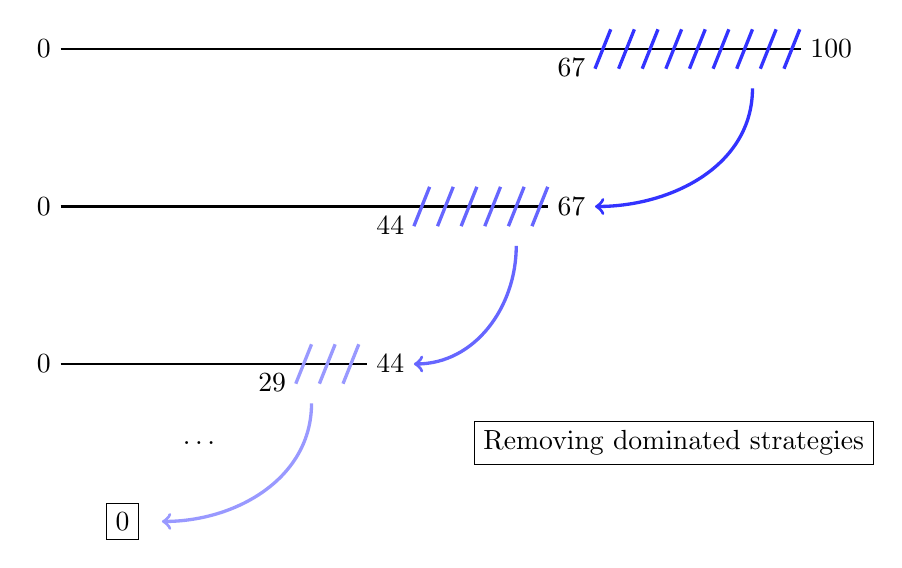
\begin{tikzpicture}
            % First level of play
            \node (0) at (0,0) {$0$};
            \node (100) at (10,0) {$100$};
            \draw [thick] (0) -- (100);
            \node [below] at (6.7,0) {$67$};

            % Getting rid of dominated strategies
            \foreach \x in {7, 7.3, 7.6, 7.9, 8.2, 8.5, 8.8, 9.1, 9.4}
            {
                \draw [blue!80, very thick] (\x,-.25) -- (\x + .2,.25);
            }
            \draw [very thick, blue!80] (9, -.5) edge[out=270,in=0,->] (7, -2);

                % Second level of play
                \node (0) at (0,-2) {$0$};
                \node (67) at (6.7,-2) {$67$};
                \draw [thick] (0) -- (67);
                \node [below] at (4.4,-2) {$44$};

                % Getting rid of dominated strategies
                \foreach \x in {4.7, 5, 5.3, 5.6, 5.9, 6.2}
                {
                    \draw [blue!60, very thick] (\x,-2.25) -- (\x + .2,-1.75);
                }
                \draw [very thick, blue!60] (6, -2.5) edge[out=270,in=0,->] (4.7, -4);

                    % Third level of play
                    \node (0) at (0,-4) {$0$};
                    \node (44) at (4.4,-4) {$44$};
                    \draw [thick] (0) -- (44);
                    \node [below] at (2.9,-4) {$29$};

                    % Getting rid of dominated strategies
                    \foreach \x in {3.2, 3.5, 3.8}
                    {
                        \draw [blue!40, very thick] (\x,-4.25) -- (\x + .2,-3.75);
                    }

                        % Final level of play
                        \node at (2, -5) {\dots};
                        \node (0) at (1,-6) [draw] {$0$};
                        \draw [very thick, blue!40] (3.4, -4.5) edge[out=270,in=0,->] (1.5, -6);

            \node at (8, -5) [draw] {Removing dominated strategies};
        \end{tikzpicture}
    \end{center}
    \caption{Equilibrium behaviour in the two thirds of the average
    game}\label{fig:rationalisation_of_two_thirds_game}
\end{figure}

The author has used this activity on a large number of occasions and at all
times collected the data. Figure \ref{fig:histogram_of_guess} shows the
distribution of the guesses (depending on the round of play):

\begin{figure}[htpb]
    \begin{subfigure}{.6\textwidth}
        \centering
        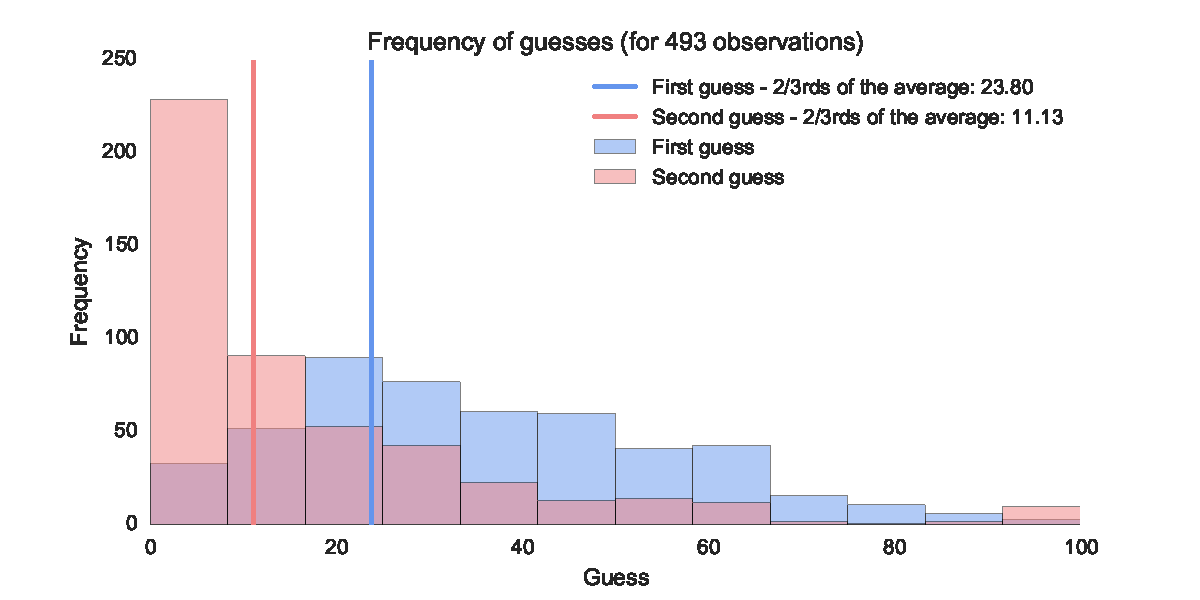
\includegraphics[width=\textwidth]{../data/histogram_of_guesses.pdf}
        \caption{Frequency of guesses depending on the round of play.}
        \label{fig:histogram_of_guess}
    \end{subfigure}
    \begin{subfigure}{.4\textwidth}
        \centering
        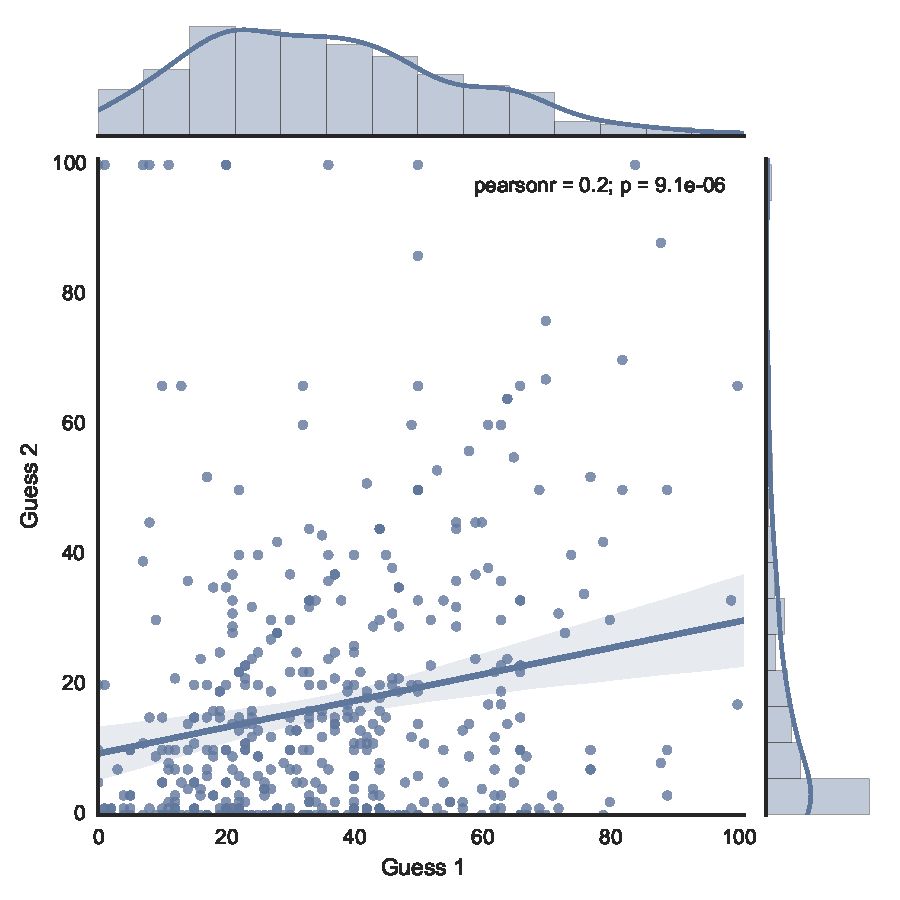
\includegraphics[width=\textwidth]{../data/jointplot_of_guesses.pdf}
        \caption{Linear relationship between guesses of each round of play.}
        \label{fig:jointplot_of_guess}
    \end{subfigure}
    \caption{Results from all data collected.}
    \label{fig:all_results}
\end{figure}

We see that the second round (after the rationalisation of play described in
Figure \ref{fig:rationalisation_of_two_thirds_game}) has guesses that are closer
to the expected equilibrium behaviour.
Figure \ref{fig:jointplot_of_guess} confirms this showing the linear
relationship (albeit a weak one with \(R^2=.2\)):

\begin{equation}
    (\text{Second guess}) = .203\times(\text{First guess}) + 9.45
    \label{eq:linear_relationship}
\end{equation}

The fact that the coefficient of the relationship is less than one highlights
that the second guess is in general lower than the first guess. As can be seen
in Figure \ref{fig:all_results} not all students reduce their guess. Figure
\ref{fig:results_with_decreasing_guess} shows the results when removing these
irrational moves. In this particular case the linear relationship is in fact
stronger \(R^2=.43\):

\begin{equation}
    (\text{Second guess}) = .33\times(\text{First guess}) + 0.20
    \label{eq:linear_relationship_for_increasing_guesses}
\end{equation}

\begin{figure}[htpb]
    \begin{subfigure}{.6\textwidth}
        \centering
        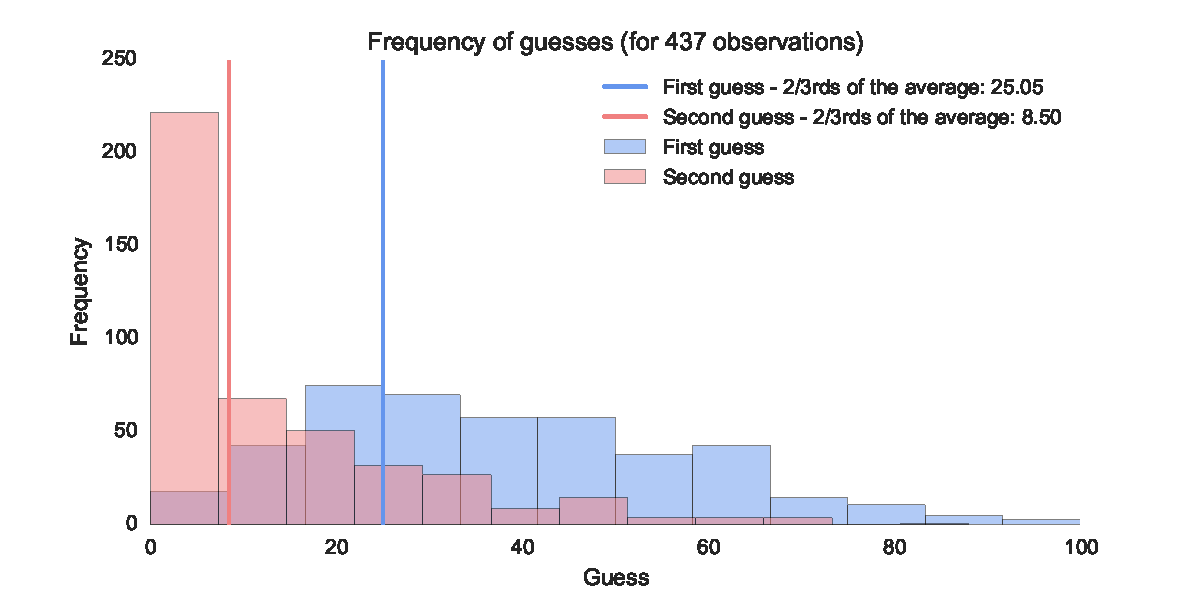
\includegraphics[width=\textwidth]{../data/histogram_of_guesses_removing_increasing_guesses.pdf}
        \caption{Frequency of guesses depending on the round of play.}
        \label{fig:histogram_of_guess}
    \end{subfigure}
    \begin{subfigure}{.4\textwidth}
        \centering
        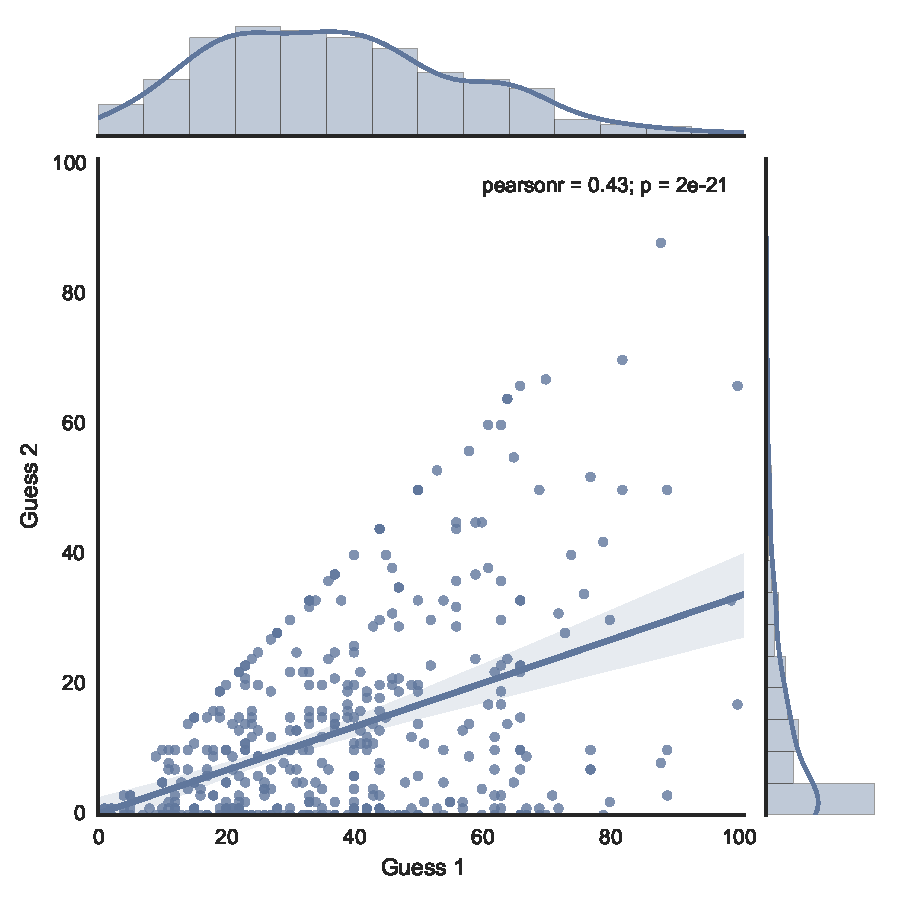
\includegraphics[width=\textwidth]{../data/jointplot_of_guesses_removing_increasing_guesses.pdf}
        \caption{Linear relationship between guesses of each round of play.}
        \label{fig:jointplot_of_guess}
    \end{subfigure}
    \caption{Results from data when removing increasing guesses.}
    \label{fig:results_with_decreasing_guess}
\end{figure}

At the end of the activity, students are shown the graphical results and a
discussion had about why the theoretic equilibrium was not the winner. This
discussion usually revolves around the observation that not everyone acted
rationally and second that some participants felt like they should `spoil' the
game by guessing larger in the second round.

Finally, if time permits (and depending on the level of the participants), the
linear relationship of (\ref{eq:linear_relationship}) is used to discuss what
would happen if more rounds were to be played. In particular it is possible to
discuss ideas of convergence when generalising (\ref{eq:linear_relationship}) to
be:

\begin{equation}
    \text{Guess}_{n+1} = .203\times\text{Guess}_n + 9.45
    \label{eq:extrapolated_linear_relationship}
\end{equation}

To summarise this activity:

\begin{enumerate}
    \item Participants are explained the rules and play one round of the two
        thirds of the average game.
    \item A rationalisation and explanation of equilibrium behaviour is
        described.
    \item Participants play another round.
    \item Results are analysed and discussed.
\end{enumerate}

This activity is still quite passive in terms of physical activity (participants are
seated throughout). Nevertheless it allows the data used for the discussion of
the theory to come directly from the participants.

\subsection{Repeated and random games}\label{sec:repeated_games}

\begin{itemize}
    \item The theory
    \item Tournaments:
        \begin{itemize}
            \item Basic type.
            \item Infinitely repeated game.
            \item Markov games.
        \end{itemize}
\end{itemize}


\section{Summary}

\begin{itemize}
    \item Give some examples of feedback.
    \item Mention how methods could be applied to other courses.
    \item Certain class management ideas (mainly that I will not speak first a
        lot of the time) <- Not sure if this is useful.
\end{itemize}

\printbibliography
\end{document}
